% !TEX root = ../SCXMLREF.tex

\subsection{iUML-B State-machines}
\label{sec:iumlb}

\iUMLB provides a diagrammatic modelling notation for \eventB in the form of state-machines and class diagrams. The diagrammatic models are contained within an \eventB machine and generate or contribute to parts of it. For example a state-machine will automatically generate the \eventB data elements (sets, constants, axioms, variables, and invariants) to implement the states while \eventB events are expected to already exist to represent the transitions. Transitions contribute further guards and actions representing their state change, to the events that they elaborate. A choice of two alternative translation encodings are supported by the iUML-B tools.  State-machines are typically refined by adding nested state-machines to states.

Figure~\ref{fig:iumlb-sm} shows an example of a state-machine, named \Bmch{SM}.
\begin{figure}[!htbp]
	\centering
	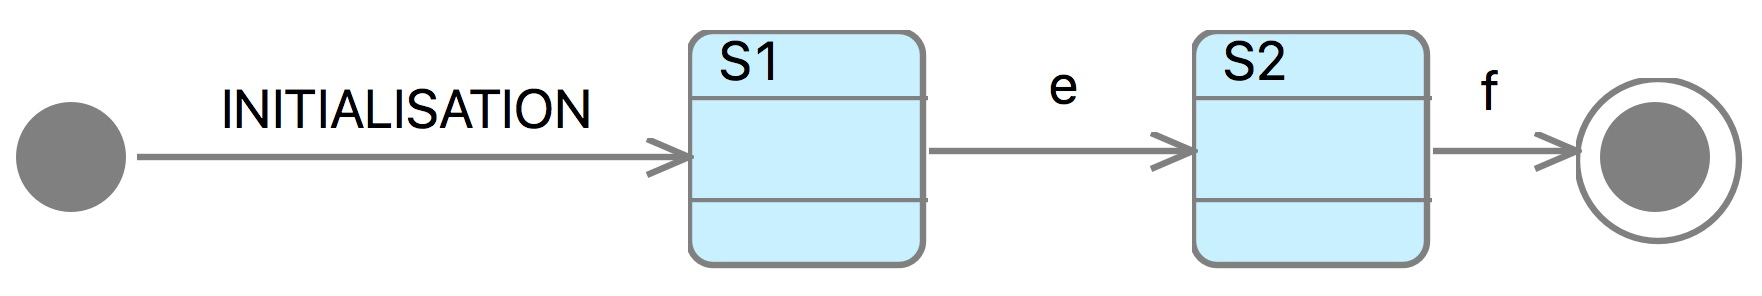
\includegraphics[width=0.8\textwidth]{figures/iumlb-SM}
	\caption{An example \iUMLB state-machine \Bmch{SM}}
	\label{fig:iumlb-sm}
\end{figure}
Here we show a translation of state-machine \Bmch{SM} using the \emph{enumeration} encoding, where each state is encoded as a constant from an enumerated set \BSMSTATES.  Variable \BSM, which represents the current state of the state-machine, is initialised to \BSI. Events \Be and \Bf change the value of \BSM according to the transitions in the state-machine.  The Event-B translation can be seen below.
\begin{Bcode}
	$\carriersets{\BSMSTATES}$ \Bhspace $\constants{\BSMNULL, \BSI, \BSII}$ \Bvspace
	$\axioms{\partition(\BSMSTATES, \BSMNULL, \BSI, \BSII)}$ \Bvspace
	$\variables{\BSM}$ \Bhspace $\invariants{\BSM \in \BSMSTATES}$ \Bvspace
	$\event{INITIALISATION}{}{}{}{}{\BSM \bcmeq \BSI}$ \Bhspace
	$\event{\Be}{}{}{\BSM = \BSI}{}{\BSM \bcmeq \BSII}$ \Bhspace
	$\event{\Bf}{}{}{\BSM = \BSII}{}{\BSM \bcmeq \BSMNULL}$
\end{Bcode}
